\subsection{Opret Projekt}\label{sec:Opretprojekt}
Dette afsnit indeholder en gennemgang af den grafisk brugergrænseflade, design og implementering af 'Opret Projekt' viewet i Rambøll Tilsyn.

\subsubsection{Design}
På Figur \ref{fig:OpretProjektSekvens} ses sekvensdiagrammet for opret bruger viewet til Rambøll Tilsyn.
\begin{figure}[H] % (alternativt [H])
	\centering
	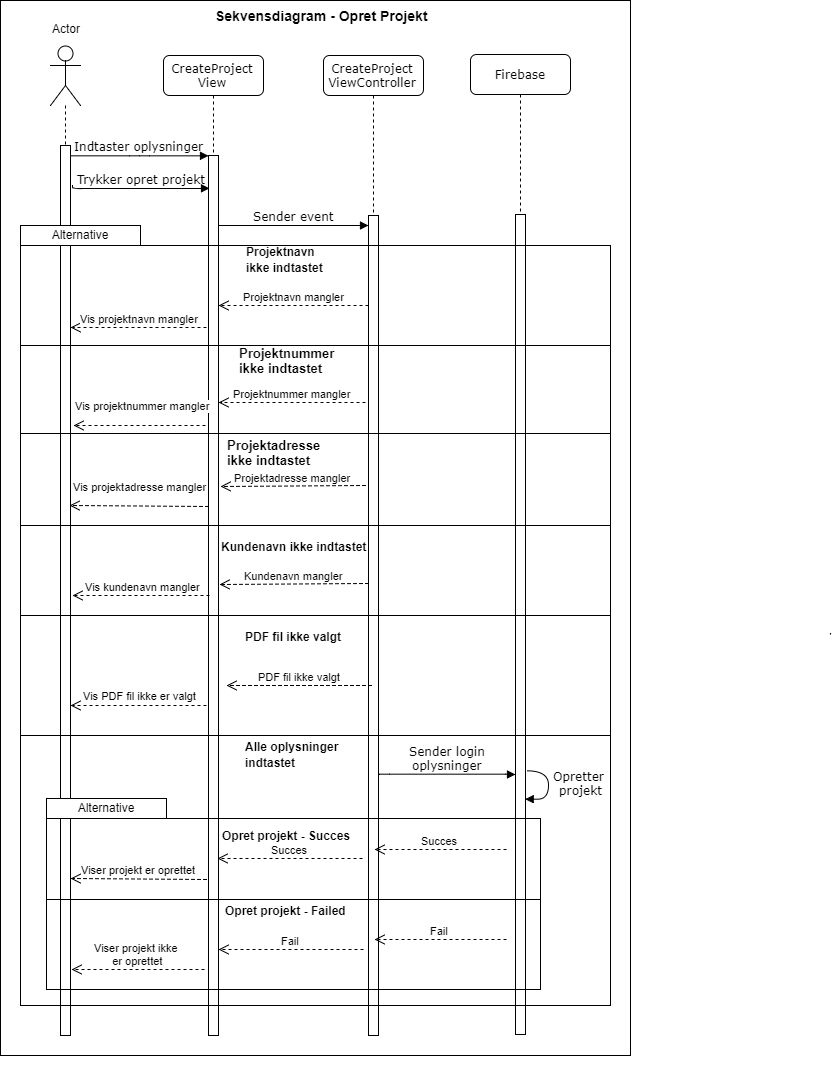
\includegraphics[height=20cm, width=15cm]{../ArkitekturDesign/Design/OpretProjekt/OpretProjektSekvensDiagram}
	\caption{Sekvensdiagram for 'Opret projekt' i Rambøll Tilsyn.}
	\label{fig:OpretProjektSekvens}
\end{figure}

\subsubsection{Grafisk brugergrænseflade}
I OpretProjektViewet er der lavet felter til alt det information, som skal tastes ind om et projekt. Se Figur \ref{fig:OpretProjektView}
\begin{figure}[H] % (alternativt [H])
	\centering
	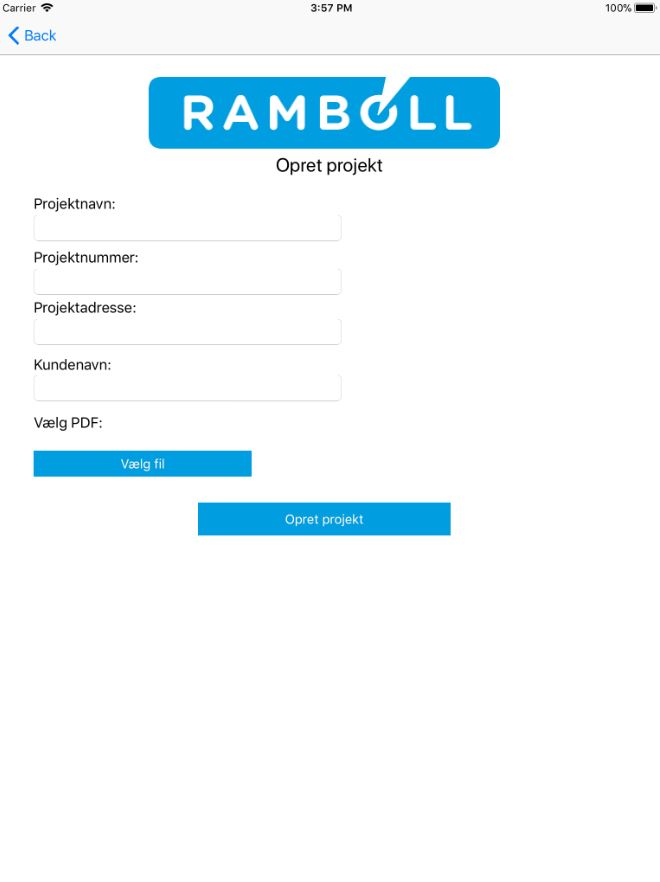
\includegraphics[height=12cm, width=10cm]{../ArkitekturDesign/Design/OpretProjekt/OpretProjektView}
	\caption{'Opret projekt' viewet som det er implementeret i Rambøll Tilsyn.}
	\label{fig:OpretProjektView}
\end{figure}

\subsubsection{Implementering}
Denne funktionalitet er ikke implementeret.

\clearpage